\documentclass{article}
\usepackage[dblblindworkshop]{neurips_2026}
\workshoptitle{AgenticOS @ NeurIPS 2026}
\usepackage[utf8]{inputenc}
\usepackage[T1]{fontenc}
\usepackage{hyperref}
\usepackage{url}
\usepackage{booktabs}
\usepackage{amsfonts}
\usepackage{amsmath}
\usepackage{nicefrac}
\usepackage{microtype}
\usepackage{xcolor}
\usepackage{graphicx}
\usepackage{enumitem}
\usepackage{tikz}
\usetikzlibrary{positioning, arrows.meta, fit, calc}
\usepackage{multicol}
\usepackage{caption}
\newcommand{\hal}{\textsc{hal}}
\title{Observability Debt in Agent Evaluation:\\
What a Telemetry Layer for Agentic OS Must Capture}
\author{Anonymous Author(s)}
\begin{document}
\small
\maketitle

\begin{abstract}
Agentic AI systems are evaluated today through three disjoint public infrastructures---leaderboards, trace corpora, and telemetry logs---none of which jointly exposes the fields a resource-aware operating layer would need: task identity, model identity, scaffold identity, outcome, token/cache usage, retries, latency, and billing. We treat this fragmentation as an empirical object and measure its consequences across three studies on public agent-evaluation data. First, using the Holistic Agent Leaderboard (\hal{}), we show that raw dollar-cost rankings transfer across some benchmark pairs (Spearman $\rho{=}0.74$--$0.93$) but are largely explained by a stable label-level cost propensity (pooled model $R^2{=}82.0\%$); success-adjusted cost is markedly less portable (mean $\rho{=}0.59$ vs.\ $0.84$). Second, using 977 exact task--model--matched trajectory pairs from Open-SWE-Traces, we show that scaffold choice changes observable execution burden at fixed task and model (OpenHands/SWE-agent turn ratio $0.85$, $[0.82, 0.87]$) and that the widely assumed ``expensive failure'' premium is not detected under exact task matching ($80\%$-power threshold: premium fractions $\geq 0.65$; observed $0.47$--$0.53$). Third, auditing two independent telemetry corpora ($8{,}058$ and $1{,}017$ sessions), we characterize the resource anatomy---$93.7\%$ mean cache-read share, $4.29{\times}$ conditional tool-error cascades, top-$1\%$-of-sessions holding $48.3\%$ of input-token volume---that a scheduler or router would need but that no benchmark currently attaches to an outcome. Together, these studies show that every unconditioned aggregate computable from today's public data conflates \emph{which workloads were attempted} with \emph{how agents behaved on them}. We specify the minimal joint telemetry schema this evidence implies and argue it belongs at the operating-system layer.
\end{abstract}

%% ============================================================
\section{Why This Belongs at the OS Layer}
\label{sec:os-layer}
%% ============================================================

Agentic AI systems increasingly persist state, invoke tools, retry failed actions, and accumulate context across long horizons. Reasoning about their resource behavior---for scheduling, routing, cost budgeting, or governance---requires the same kind of unified telemetry that operating systems have long provided for conventional workloads: a common schema linking \emph{what ran}, \emph{on what}, \emph{under which policy}, \emph{with what outcome}, and \emph{at what resource cost}. No such schema currently exists for agentic AI, and we show empirically that its absence is the dominant source of noise in every cost signal practitioners currently rely on.

We treat three public data sources as stand-ins for what an agentic OS's observability layer would need to unify: a cost-and-outcome leaderboard (\hal{}), a task/model/scaffold-matched trajectory corpus (Open-SWE-Traces), and raw session-level usage telemetry (two independent corpora). Each exposes a different partial view. \hal{} links dollar cost to outcome but encrypts execution traces. Open-SWE-Traces exposes exact task/model/scaffold matching and resolved status but no tokens or billing. The telemetry corpora expose token, cache, and tool-call dynamics but no task outcome or billing. \textbf{No public source jointly exposes task, model, scaffold, outcome, token/cache usage, retries, latency, and billing}---the minimal schema a resource-aware agentic OS layer needs.

%% ============================================================
\section{Related Work}
\label{sec:related}
%% ============================================================

Kapoor et al.\ (2026) introduce \hal{} as cost-aware evaluation infrastructure spanning coding, web, science, and customer-service tasks, reporting 21,730 rollouts and roughly \$40,000 in evaluation cost. Kapoor et al.\ (2024) motivate joint accuracy--cost reporting and convex-hull frontier analysis, which we adopt as one of three decision-frontier definitions. Ndzomga (2026) asks whether task subsets preserve agent rankings within a single benchmark; we instead ask whether an \emph{observed cost signal} predicts a \emph{different} workload. Benchmark$^2$ studies cross-benchmark rank consistency for static LLM benchmarks; our setting adds interactive scaffolds, dollar cost, success adjustment, and a held-out workload test. SWE-Effi reports that failed attempts consume substantially more resources than successful ones; our matched design tests that claim at fixed task and does not detect the premium once task-difficulty confounding is removed (Section~\ref{sec:matched}). Open-SWE-Traces supplies the exact task/model matching that makes this test possible but does not expose token or billing fields, motivating the schema argument in Section~\ref{sec:schema}.

%% ============================================================
\section{Study 1: Does a Cost Signal Travel?}
\label{sec:cost}
%% ============================================================

\subsection{Data and cohort}

We use the public \texttt{all\_leaderboards\_costs\_HAL.csv} snapshot: 242 displayed evaluations across nine benchmarks, 11 scaffolds, and 29 displayed model labels. The CSV supplies accuracy and aggregate dollar cost but no token components, provider aliases, tool-call counts, retry counts, or per-task trajectories. Fixing the displayed \hal{} Generalist Agent scaffold and matching exact model-label strings yields six workloads with adequate repeated-label overlap for a cohort of 86 rows and 25 displayed labels.

\subsection{Raw cost transfers; the mechanism does not}

Across six benchmark pairs with $\geq 12$ shared labels, raw dollar-cost Spearman $\rho$ ranges from $0.74$ to $0.93$ (mean $0.84$), surviving Holm-corrected permutation testing. A pooled label-plus-benchmark log-cost fixed-effects model explains $R^2 = 82.0\%$ (adjusted $72.7\%$) of observed cost variation. Critically, once benchmark and displayed-label cost propensity are removed, \textbf{no high-overlap residual-cost rank association survives} a 20,000-draw permutation test.

\begin{figure}[t]
\centering
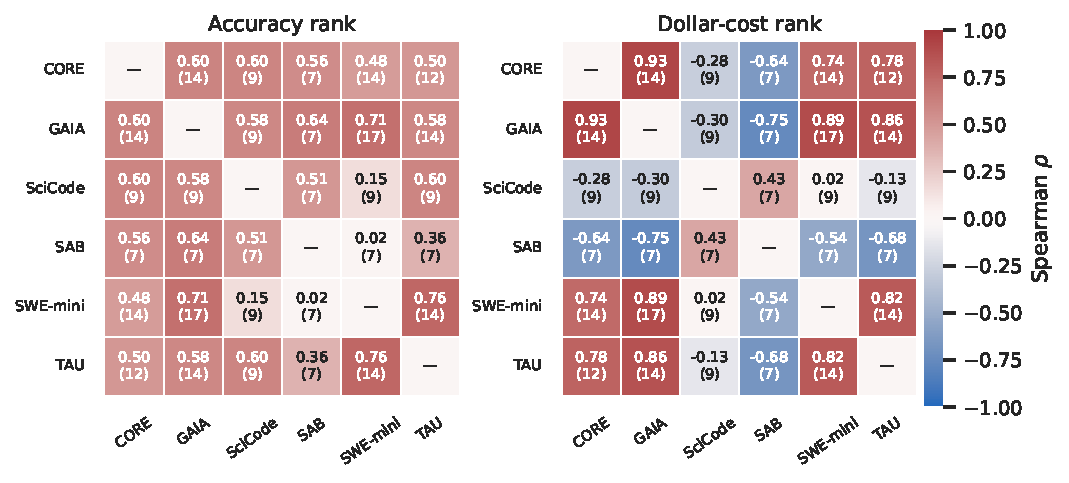
\includegraphics[width=0.85\linewidth]{figures/rank_transfer_compact.pdf}
\caption{\textbf{Cost-rank transfer.} Pairwise Spearman correlations for raw dollar cost (left) and cost per success (right) across six benchmark pairs with $\geq 12$ shared labels. Raw cost is strongly portable; CPS is not.}
\label{fig:rank_transfer}
\end{figure}

Leave-one-benchmark-out (LOBO) prediction succeeds for CORE ($\rho{=}0.78$, $N{=}14$), GAIA ($0.87$, $N{=}16$), SWE-mini ($0.90$, $N{=}16$), and TAU ($0.83$, $N{=}14$), all $p < 0.005$. It fails for SciCode (unstable, $[-0.50, 0.14]$) and ScienceAgentBench (directionally negative, $[-0.77, -0.43]$).

\textbf{Interpretation for an OS layer:} the portable component of raw cost is a stable, label-level propensity---plausibly provider pricing, reasoning-mode defaults, or routing policy---that a router could in principle learn and reuse. But the public data cannot identify \emph{which} mechanism it is, because none of the distinguishing fields (token components, routing decisions, cache treatment) are exposed.

\subsection{Success-adjusted cost is a different, less portable ranking}

Cost per expected success, $\text{CPS}_{i,b}(\epsilon) = C_{i,b} / \max(A_{i,b}, \epsilon)$ with $\epsilon = 0.01$, has mean Spearman $\rho = 0.59$ versus $0.84$ for raw cost. Only three pairs survive permutation testing and Holm correction: CORE--GAIA ($\rho{=}0.87$, $[0.63, 0.96]$), CORE--TAU ($0.83$, $[0.31, 1.00]$), and GAIA--TAU ($0.78$, $[0.42, 0.94]$). The clearest gap is GAIA--SWE-mini ($0.60$, $[0.14, 1.13]$): a label cheap in raw dollars is not reliably cheap per expected success elsewhere.

%% ============================================================
\section{Study 2: Matched Trajectories}
\label{sec:matched}
%% ============================================================

\hal{}'s own trace archives are encrypted, so Study~1 cannot say \emph{why} costs differ. We therefore use a separate, external, unencrypted trace corpus---977 exact task--model pairs from Open-SWE-Traces for MiniMax-M2.5 under two scaffolds, OpenHands and SWE-agent. The schema exposes resolved status, message roles, tool calls, and text, but not billed tokens, dollars, or latency; we treat turns, tool calls, and character counts as trace-burden proxies.

\subsection{Scaffold choice changes observable burden}

At fixed task and model, OpenHands has lower matched medians: $123$ vs.\ $149$ trajectory turns (ratio $0.85$, $[0.82, 0.87]$), $61$ vs.\ $74$ tool calls ($0.85$, $[0.82, 0.86]$), and $176{,}708$ vs.\ $194{,}263$ characters ($0.95$, $[0.92, 0.98]$). Resolved status shows no detected difference ($p{=}0.197$).

\begin{figure}[t]
\centering
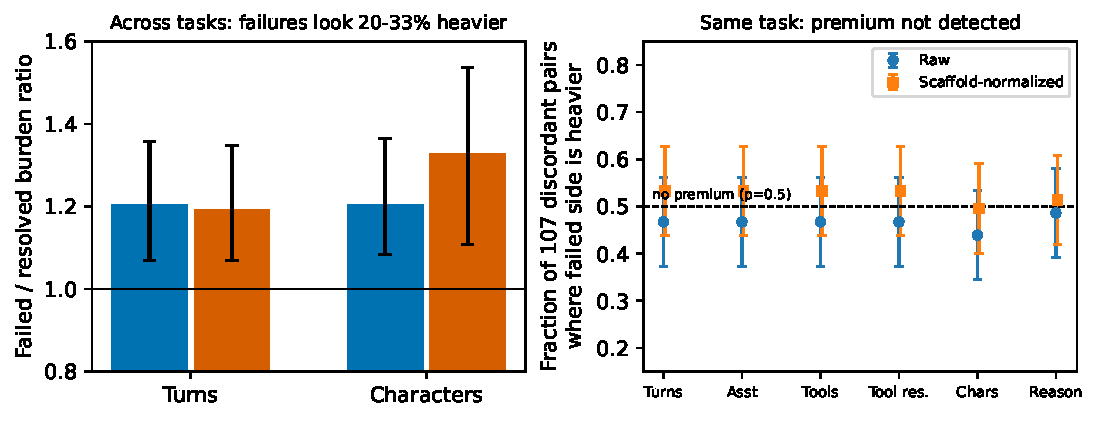
\includegraphics[width=0.85\linewidth]{figures/failure_burden_discordant.pdf}
\caption{\textbf{Failure-cost premium dissolves under exact task matching.} Left: naive cross-task ratios (failed/resolved) reproduce the ``expensive failure'' folklore. Right: among 107 discordant pairs (same task, one scaffold resolved, the other failed), the failed side is heavier only $47$--$52/107$ on every metric.}
\label{fig:failure_burden}
\end{figure}

\subsection{The ``expensive failure'' premium is a composition artifact}

Comparing failed vs.\ resolved trajectories \emph{across} tasks reproduces the folklore ($19$--$36\%$ heavier failures). But among \textbf{107 discordant pairs}---identical task, identical model, one scaffold resolved and the other failed---the failed side is heavier only $47$--$52$ times out of $107$ on every metric (two-sided binomial $p \geq 0.25$). Normalizing by each scaffold's median gives a failed/resolved ratio of $0.98$--$1.06$ with intervals spanning $1$. A power calculation shows $80\%$ power to detect a premium fraction $\geq 0.65$; the observed $0.47$--$0.53$ rules out strong versions but not modest ones.

\textbf{Interpretation for an OS layer:} hard tasks make agents both burn more and fail. An unconditioned failure-cost multiplier measures \emph{which tasks were attempted}, not a causal property of failing runs. Task-conditioned accounting requires exactly the joint task/model/scaffold/outcome schema that no single public source provides.

%% ============================================================
\section{Study 3: Telemetry Anatomy}
\label{sec:telemetry}
%% ============================================================

Sections~\ref{sec:cost}--\ref{sec:matched} show that cost and failure aggregates are confounded by workload composition. This section asks: what does raw execution telemetry look like, and how far do public sources go toward exposing it?

We audit two independent coding-agent telemetry corpora. \textbf{TraceLab} contributes $8{,}058$ real-world sessions ($665{,}453$ LLM rounds, $743{,}819$ tool calls). \textbf{MIMO Claude Code} contributes $1{,}017$ sessions ($4{,}690$ rounds) from a single model. Neither links usage to task outcome or billing.

\subsection{Context is the dominant resource}

In TraceLab, the median round carries $132{,}092$ input tokens against only $249$ output tokens, with a $93.7\%$ mean cache-read share; median final-round context is $3.6{\times}$ the initial round (P90 $9.9{\times}$). A single dollar total on a leaderboard row cannot distinguish spending driven by model price from spending driven by cache policy or context accumulation.

\begin{figure}[t]
\centering
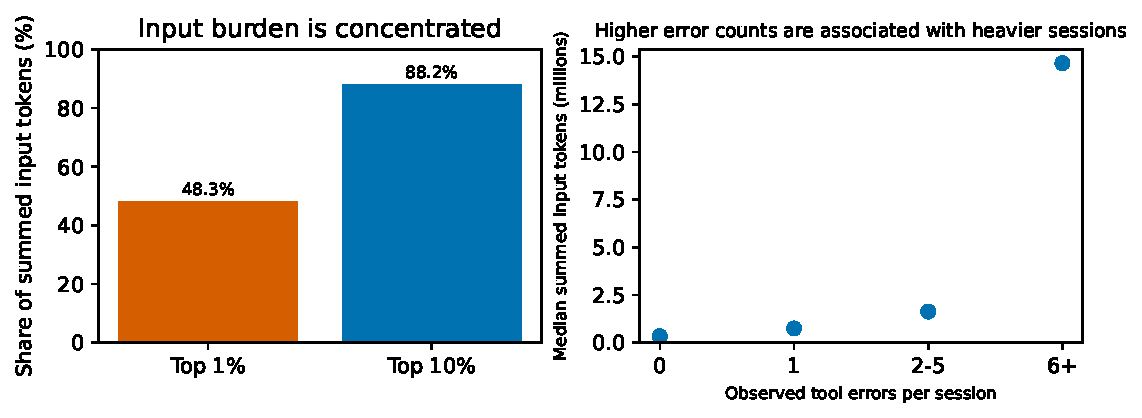
\includegraphics[width=0.85\linewidth]{figures/tracelab_tail_error_burden.pdf}
\caption{\textbf{Resource burden is heavy-tailed.} Top $1\%$ of TraceLab sessions hold $48.3\%$ of summed input-token volume; top $10\%$ hold $88.2\%$. Median input rises from $0.34$M tokens at zero errors to $14.65$M at six or more.}
\label{fig:telemetry_tail}
\end{figure}

\subsection{Error cascades replicate across sources}

After a successful tool call, the next call errs $4.9\%$ of the time; after an erroneous call, $21.0\%$ ($4.29{\times}$ conditional increase). MIMO replicates this almost exactly: $4.3\%$ after an error vs.\ $1.0\%$ after a success ($4.33{\times}$). Retrying is the norm ($88.3\%$ of errored calls get a same-tool retry; $77.9\%$ succeed), but the tail is pathological---consecutive-error run length has median $1$, P90 $3$, max $368$.

\subsection{Data-quality boundary}

Every released MIMO session repeats one constant per-round usage tuple, so within-session token dynamics cannot be validated; we restrict MIMO to session counts, corpus totals, cross-session concentration, and content-derived error sequences.

%% ============================================================
\section{The Minimal Joint Schema}
\label{sec:schema}
%% ============================================================

Based on the empirical gaps above, we specify the minimal joint schema a shared observability layer needs per execution unit, tying each field to the OS-layer function it unblocks:

\begin{enumerate}[nosep,leftmargin=1.5em]
\item \textbf{Task and model identity} (exact, not display-label strings)---required for any exact-matched comparison; without it, the failure-premium test in Section~\ref{sec:matched} would be impossible.
\item \textbf{Scaffold/harness identity and version}---required to attribute burden differences to scaffold design rather than model behavior, directly relevant to routing.
\item \textbf{Outcome/resolved status}---required to condition cost statistics on success, closing the CPS-portability gap in Section~\ref{sec:cost}.
\item \textbf{Token components (input, output, cache-read, cache-creation) per round}---required to distinguish price from context-accumulation and cache-policy effects (Section~\ref{sec:telemetry}).
\item \textbf{Tool-call counts, retries, and error status per call}---required to detect and price error-cascade dynamics ($4.29{\times}$ conditional increase), relevant to a governance layer deciding when to halt a spiraling session.
\item \textbf{Latency per call and per session}---absent from every source audited; required for real-time scheduling.
\item \textbf{Billing, linked to the above}---the only field \hal{} exposes well, and precisely the field that becomes uninterpretable without the others.
\end{enumerate}

\begin{figure}[t]
\centering
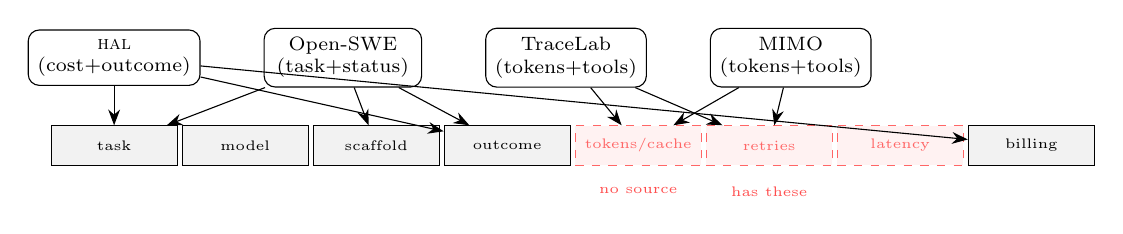
\begin{tikzpicture}[
  node distance=0.6cm and 0.8cm,
  source/.style={draw, rounded corners, minimum width=2cm, minimum height=0.7cm, font=\scriptsize, align=center},
  field/.style={draw, minimum width=1.6cm, minimum height=0.5cm, font=\tiny, align=center, fill=gray!10},
  gap/.style={draw, dashed, red!60, minimum width=1.6cm, minimum height=0.5cm, font=\tiny, align=center, fill=red!5},
  arr/.style={-{Stealth[length=2mm]}, thin}
]
\node[source] (hal) {\hal{}\\(cost+outcome)};
\node[source, right=of hal] (swe) {Open-SWE\\(task+status)};
\node[source, right=of swe] (tl) {TraceLab\\(tokens+tools)};
\node[source, right=of tl] (mimo) {MIMO\\(tokens+tools)};

\node[field, below=0.5cm of hal] (f1) {task};
\node[field, right=0.05cm of f1] (f2) {model};
\node[field, right=0.05cm of f2] (f3) {scaffold};
\node[field, right=0.05cm of f3] (f4) {outcome};
\node[gap, right=0.05cm of f4] (f5) {tokens/cache};
\node[gap, right=0.05cm of f5] (f6) {retries};
\node[gap, right=0.05cm of f6] (f7) {latency};
\node[field, right=0.05cm of f7] (f8) {billing};

\draw[arr] (hal) -- (f1);
\draw[arr] (hal) -- (f4);
\draw[arr] (hal) -- (f8);
\draw[arr] (swe) -- (f1);
\draw[arr] (swe) -- (f3);
\draw[arr] (swe) -- (f4);
\draw[arr] (tl) -- (f5);
\draw[arr] (tl) -- (f6);
\draw[arr] (mimo) -- (f5);
\draw[arr] (mimo) -- (f6);

\node[below=0.15cm of f5, font=\tiny, text=red!70] {no source};
\node[below=0.15cm of f6, font=\tiny, text=red!70] {has these};
\end{tikzpicture}
\caption{\textbf{The observability gap.} Each public source exposes a different partial slice of the joint schema. Red dashed boxes mark fields no source provides. Only the joint schema (all eight fields together) unblocks task-conditioned cost accounting and resource-aware scheduling.}
\label{fig:schema}
\end{figure}

No existing public release exposes this joint schema. We do not propose a specific storage format or API---that is a systems-design question outside this paper's scope---but we argue, from the measured consequences of its absence, that this schema belongs at a shared operating-system layer rather than being re-derived piecemeal inside each benchmark.

%% ============================================================
\section{Limits}
\label{sec:limits}
%% ============================================================

This is a secondary-data analysis. Public display labels do not fully identify prompts, tools, budgets, harness versions, or routing; the \hal{} cohort is sparse, unbalanced, and mostly single-run. Cost-propensity adjustment is an observational fixed-effects decomposition, not provider-list-price control. CPS is an aggregate ratio, not the mean cost of successful runs. The Open-SWE extension uses one model and a nonrandom four-shard boundary sample; its proxies are not tokens or dollars, and the failure-premium null is powered to rule out strong effects ($\geq 15$pp) but not modest ones. The telemetry audit does not link to task success or billing; MIMO's per-round usage fields cannot be independently verified. None of these limits invalidate the schema argument---each is itself an instance of the missing-field problem.

%% ============================================================
\section{Conclusion}
\label{sec:conclusion}
%% ============================================================

Three independent studies converge on the same structural finding: raw cost, success-adjusted cost, and failure-cost premiums are all measurably confounded by information that today's fragmented evaluation infrastructure does not expose jointly. Raw cost transfers across some workloads but mostly reflects stable label-level pricing. Success adjustment reorders the ranking and survives correction for only half the tested pairs. A widely assumed failure-cost premium is not detected once task difficulty is held fixed. Underlying all three results is a single missing artifact: no public source jointly links task, model, scaffold, outcome, token/cache usage, retries, latency, and billing. We specify that schema and argue it is properly a function of a shared operating-system layer for agentic AI---the same role a conventional OS's resource-accounting subsystems play for compute workloads---rather than something each leaderboard should attempt to reconstruct independently.

%% ============================================================
\section*{Checklist}
%% ============================================================

\begin{itemize}[nosep,leftmargin=1.5em]
\item[\textbf{1.}]\textbf{Claims:} All claims are supported by empirical analysis on public data. No new benchmark or estimator is proposed.
\item[\textbf{2.}]\textbf{Data:} All data sources are public. HAL CSV distributed with Ndzomga (2026). Open-SWE-Traces from NVIDIA. TraceLab and MIMO are public telemetry corpora.
\item[\textbf{3.}]\textbf{Code:} Analysis scripts will be released upon acceptance. Results are reproducible from public data.
\item[\textbf{4.}]\textbf{Anonymization:} This submission is double-blind. No identifying information is included.
\item[\textbf{5.}]\textbf{Limitations:} Section~\ref{sec:limits} discusses construct boundaries, sample constraints, and power limitations.
\item[\textbf{6.}]\textbf{Societal impact:} This work improves evaluation infrastructure; no direct societal harm is identified.
\end{itemize}

%% ============================================================
\bibliographystyle{plainnat}
\begin{thebibliography}{10}

\bibitem[Ahmad et~al.(2026)]{ahmad2026open}
Wasi~Uddin Ahmad, Nikolai Ludwig, Somshubra Majumdar, and Boris Ginsburg.
\newblock Open-{SWE}-traces: Advancing dual-mode multilingual distillation for
  software engineering agents.
\newblock {\em arXiv preprint arXiv:2606.16038}, 2026.

\bibitem[Fan et~al.(2025)]{fan2025sweeffi}
Zhiyu Fan, Kirill Vasilevski, Dayi Lin, et~al.
\newblock {SWE}-effi: Re-evaluating software {AI} agent system effectiveness
  under resource constraints.
\newblock {\em arXiv preprint arXiv:2509.09853}, 2025.

\bibitem[Kapoor et~al.(2024)]{kapoor2024agents}
Sayash Kapoor et~al.
\newblock {AI} agents that matter.
\newblock {\em arXiv preprint arXiv:2407.01502}, 2024.

\bibitem[Kapoor et~al.(2026)]{kapoor2026hal}
Sayash Kapoor et~al.
\newblock Holistic agent leaderboard: The missing infrastructure for {AI} agent
  evaluation.
\newblock {\em arXiv preprint arXiv:2510.11977}, 2026.

\bibitem[Ndzomga(2026)]{ndzomga2026efficient}
Franck Ndzomga.
\newblock Efficient benchmarking of {AI} agents.
\newblock {\em arXiv preprint arXiv:2603.23749}, 2026.

\bibitem[Qian et~al.(2026)]{qian2026benchmark2}
Qi Qian, Chengsong Huang, et~al.
\newblock Benchmark$^2$: Systematic evaluation of {LLM} benchmarks.
\newblock {\em arXiv preprint arXiv:2601.03986}, 2026.

\end{thebibliography}

\end{document}
